%%%%%%%%%%%%%%%%%%%%%%%%%%%%%%%%%%%%%%%%%%%%%%%%%%%%%%%%%%%%%%%%%%%%%%%%%%%%%%%%%%%%%%%%%%%%%%%%%%%%
% ==================================================================================================
% --------------------------------------------------------------------------------------------------
\chapter{Introduction}
Digitization of medical imaging has facilitated innumerable advances in disease understanding and treatment. From multi-modal image fusion to image guided therapy, software tools now underpin research and clinical workflows in almost every domain of medical imaging.
\par
This work concerns an unsolved segmentation problem in 3D brain magnetic resonance imaging (MRI), in which the objective is to automatically predict the class, or label, of every voxel (``volume pixel'') in the image. The objects of interest are white matter hyperintensities (WMH), non-cancerous brain lesions which are correlated with several neurodegenerative diseases. This chapter presents the motivation for automated WMH segmentation, gives a problem definition, and explores the previously proposed solutions.
%%%%%%%%%%%%%%%%%%%%%%%%%%%%%%%%%%%%%%%%%%%%%%%%%%%%%%%%%%%%%%%%%%%%%%%%%%%%%%%%%%%%%%%%%%%%%%%%%%%%
\section{Background}
The brain is composed of three major classes of tissue: grey matter (GM), white matter (GM), and cerebrospinal fluid (CSF). Grey matter constitutes the peripheral surface of the brain -- the cortex, approximately 5mm thick -- as well as some deeper structures called the basal ganglia. It contains neuronal cell bodies, and performs the bulk of neural processing. The white matter is composed primarily of myelinated axons, and functions to relay information between different GM structures in the brain. The brain is surrounded by CSF, which provides mechanical and immunological defence. It is produced by the choroid plexuses in the ventricles of the brain -- a series of 4 connected cavities.
% ==================================================================================================
\subsection{Magnetic Resonance Imaging}\label{ss:mri}
Magnetic resonance imaging (MRI) provides superior and flexible brain tissue contrast versus computed tomography (CT) imaging, and is the primary modality for imaging brain disease. Whereas CT measures tissue density via attenuation of transmitted X-rays, which does not vary significantly among brain tissues, MRI measures a mutable combination of 3 tissue characteristics: the proton density (PD)\footnote{MRI can be used to image any nucleus with a net nuclear dipole, but proton (hydrogen) imaging is most common since hydrogen is biologically abundant and gives a strong signal intensity.}, and T1 and T2 relaxation constants \cite{Pooley2005}. The physics of signal generation are described below.
\par
\begin{figure}[b]
  \centering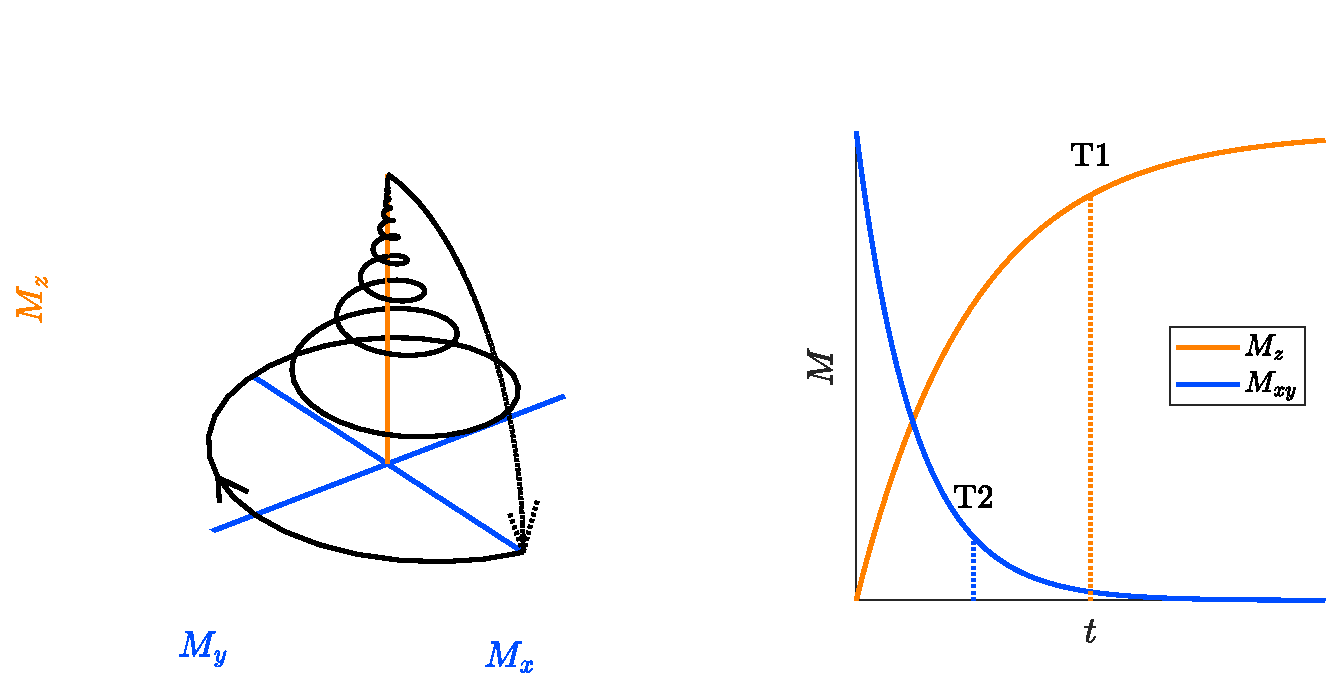
\includegraphics[width=\plotwidth]{mridecay3d}
  \caption{Visualization of T1 and T2 relaxation.}
  \label{fig:mridecay3d}
\end{figure}
In an MR scanner, a powerful magnetic field induces alignment of proton dipoles with the field. Only a tiny fraction of the total protons align, but they create a small magnetic field $M_z$ which is distinct from the main field \cite{Bloch1946}. The aligned protons also rotate about the axis of alignment, imperfectly, like a spinning top; this is called precession, and the frequency of rotation is roughly homogeneous and proportional to the main field strength \cite{Bloch1946}. If a second magnetic field is applied which is $90^{\circ}$ perpendicular to the first, and rotating at the precession frequency, the aligned protons can be forced into temporary alignment with this transverse rotating field, before decaying back towards their original state, as illustrated in Figure \ref{fig:mridecay3d} \cite{Bloch1946}. This transient applied magnetic field is induced by a radio frequency (RF) pulse, and the rate at which the original magnetization $M_z$ is regained is described by the tissue-specific T1 relaxation constant,
\begin{equation}
M_z = M_0\et\left(1-e^{-\left(\frac{t}{T1}\right)}\right)\label{eq:T1}.
\end{equation}
The T1 constant is dictated by the ability of protons in the tissue to transfer energy to bonded atoms and surrounding molecules, since this energy transfer defines the transition from the high energy transverse state to the low energy original state \cite{Bloch1946,Bryant2005}. Large macromolecules, membranes, and lipids are generally able to facilitate this energy transfer more effectively than small molecules like water, producing a shorter T1 \cite{Koenig1990}. For this reason, myelinated WM has a shorter T1 than GM, which in turn has a shorter T1 than CSF, which is mostly water \cite{Roberts2007}.
\par
The rate of decay of the transverse moment $M_{xy}$ is actually not equal to the rate of regeneration of $M_z$. Rather, this is governed by the T2 relaxation constant,
\begin{equation}
M_{xy} = M_0\et\left(e^{-\left(\frac{t}{T2}\right)}\right)\label{eq:T2},
\end{equation}
which is always shorter that T1. This is because, in addition to T1 effects, the net rotating moment $M_{xy}$ is eroded by proton dephasing. When precessing protons, having a net dipole, interact with other dipoles or charged particles, their rotational frequency can be increased or decreased, but overall less coherent, reducing the perceptible net magnetization $M_{xy}$ \cite{Bloch1946}. In highly structured tissues like GM and WM, these interactions are more variable, dephasing is faster, and T2 is shorter \cite{Roberts2007}. In fluid environments like CSF, proton interactions are more homogeneous, yielding longer T2 \cite{Roberts2007}. For this reason, T2-weighted images are especially useful in identifying pathologies which degrade tissue structure, since they will have abnormally high T2 \cite{Roberts2007}. Both relaxation constants depend in a small way on the main magnetic field strength, measured in Tesla (T); T1 and T2 values for various brain tissues at 1.5T are summarized in Table \ref{tab:t1t2tissues}.
\par
\begin{table}
  \caption{T1 and T2 constants for brain tissues at 1.5 Tesla.}
  \label{tab:t1t2tissues}
  \centering{\setlength{\tabcolsep}{2pt}
    \begin{tabular}{ccrclcrclcrclcl}\hline
      Tissue && \multicolumn{3}{c}{T1 (ms)} && \multicolumn{3}{c}{T2 (ms)} && \multicolumn{3}{c}{$K [H]$ (a.u.)}&& Ref\\\hline
      WM  &&  719 & $\pm$ &  33 &&   73 & $\pm$ &   6 && 0.81 & $\pm$ & 0.03 && \cite{Schmitt2004}\\
      GM  && 1165 & $\pm$ &  88 &&   92 & $\pm$ &  11 && 0.98 & $\pm$ & 0.07 && \cite{Schmitt2004}\\
      CSF && 3337 & $\pm$ & 111 && 2562 & $\pm$ & 123 && 1.00 & $\pm$ & 0.07 && \cite{Schmitt2004}\\
      WML && 1124 & $\pm$ & 372 &&  136 & $\pm$ &  79 &&      &  $-$  &      && \cite{Stevenson2000}\ss{a}\\
      \hline
  \end{tabular}}
  \tablepost{\ss{a} Estimated from Fig 1 supratentorial data (numerical results not given); $\pm$ IQR, not SD; cf. \S\ \ref{ss:WMD} for definition.}
\end{table}
Image acquisition involves sensing the transverse magnetization $M_{xy}$ following proton excitation by an RF pulse. The problem is that this small signal decays very quickly due to proton dephasing, which occurs even faster than $T2$ would predict due to a third factor, inhomogeneity in the main magnetic field \cite{Chavhan2009}. The time constant for this decays is termed $T2^*$, and its effects are usually undesirable \cite{Chavhan2009}. As a result, $M_{xy}$ is easily overpowered by the magnetic moment from the RF pulse, even after it is turned off, due to resonance. An important solution to this, called the spin-echo, was proposed by Erwin Hahn in \citeyear{Hahn1950} \cite{Hahn1950}. If $T2^*$ for each proton is assumed to be constant, then reversing the direction of rotation at a time $t$ should cause all protons to align again at exactly $2t$. Therefore, at $2t$ the transverse magnetization $M_{xy}$ -- the image signal -- manifests again for sensing, no longer confounded by RF coil resonance \cite{Hahn1950}.
\par
This second signal is called the Spin Echo ($SE$), and the interval $2t$ is termed the echo time ($TE$). Reversing the direction of rotation can be achieved by a $180^{\circ}$ RF pulse at time $TE/2$, in the same way the original excitation is achieved using a $90^{\circ}$ RF pulse (amount of rotation is proportional to the energy of the pulse). Acquisition of an entire image requires repetitions of this sequence with an interval called the repetition time ($TR$). An example spin echo sequence, showing $TE$ and $TR$, as well as $T1$ and $T2$ decay, is illustrated in Figure \ref{fig:mrispinecho}. Spatial encoding for creation of 2D and 3D images requires the use of additional electromagnetic gradients; however this topic is omitted here since it is quite involved, and not essential to the current work\footnote{The interested reader is directed to this comprehensive resource on the topic: \hreftt{http://mri-q.com/}}.
\par
\begin{figure}
  \centering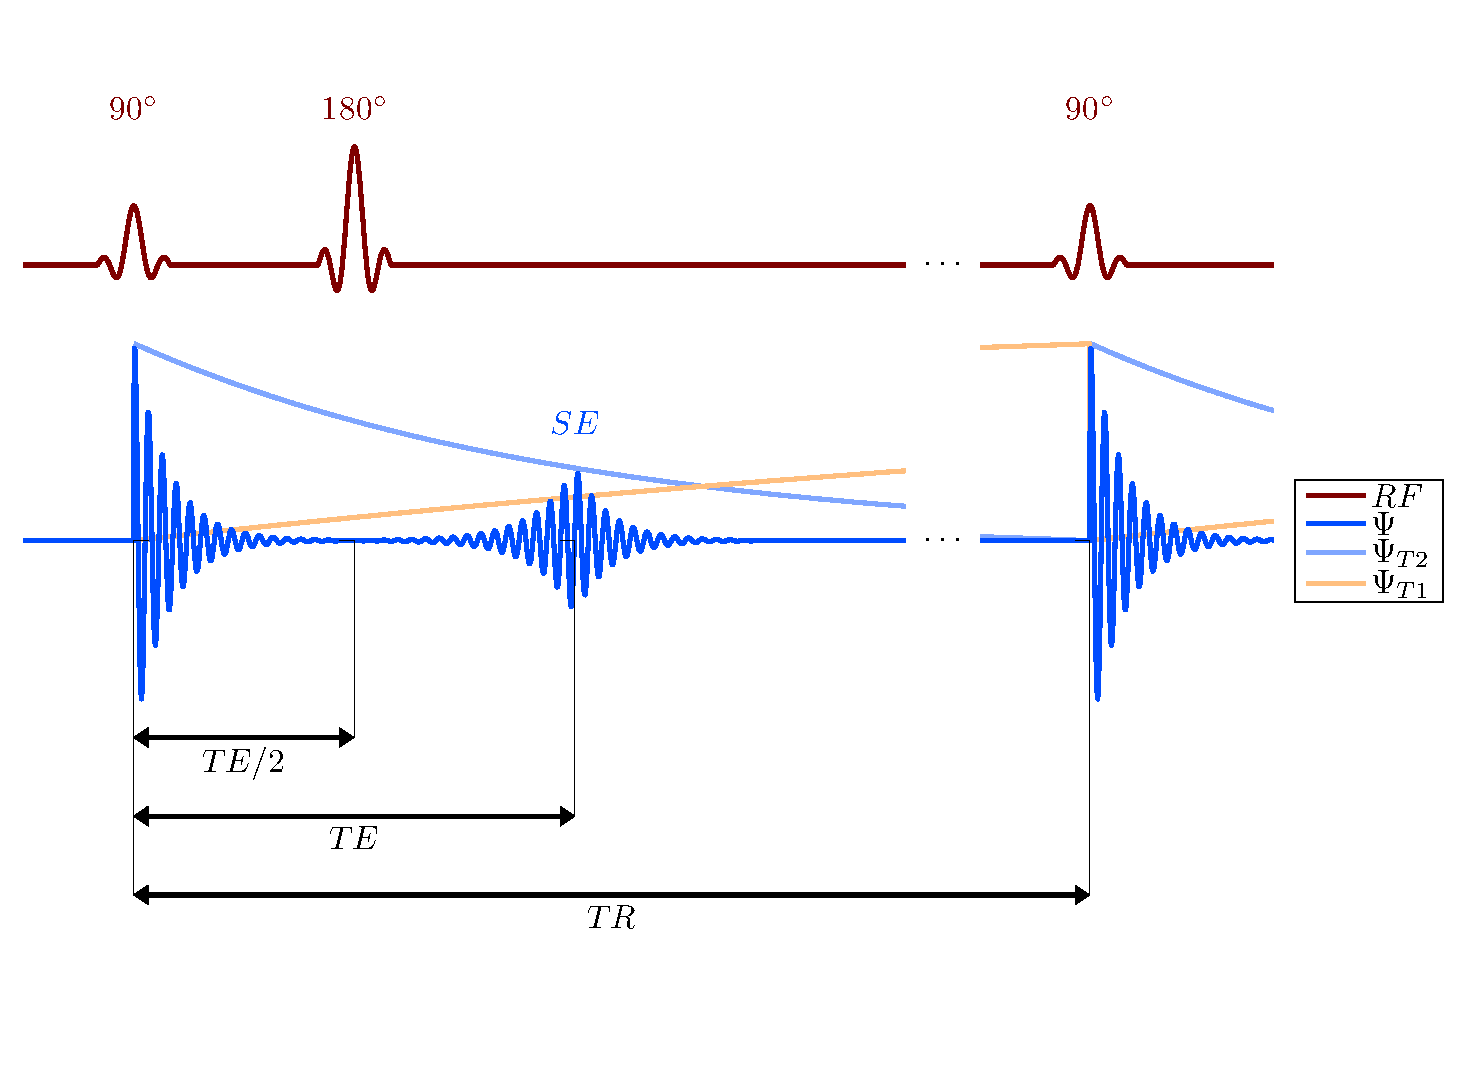
\includegraphics[width=\plotwidth]{mrispinecho}
  \caption{RF and MR signal for a basic Spin Echo sequence.}
  \label{fig:mrispinecho}
\end{figure}
Using these principals, the nature of MR image contrast can finally be understood. That is, the signal intensity $\Psi$ for a spin echo sequence at location $x$ can be described by the following 3-term equation,
\begin{equation}\label{eq:MRI-SE}
\Psi_{SE}(x) = \bigg[K [H](x)\bigg]\bigg[e^{-\left(\frac{TE}{T2(x)}\right)}\bigg]\bigg[1 - e^{-\left(\frac{TR}{T1(x)}\right)}\bigg],
\end{equation}
where $K$ is scaling factor, and $\left[H\right]$ denotes the proton density. If $TR$ is chosen to be relatively long, then the longitudinal magnetization $M_z$ is allowed to recover completely after each repetition, the third term tends towards 1 for all tissues, and differences in tissue specific $T1$ are nullified. Similarly, if $TE$ is relatively short, then $M_{xy}$ has little time to dephase, the second term is maintained close to 1, and differences in $T2$ are nullified. In order to emphasize differences in $T1$, therefore, $TR$ can be chosen shorter; for $T2$-weighted contrast, $TE$ can be chosen longer; and if differences in $[H]$ (proton density, PD) are to be emphasized, $TR$ can be kept long and $TE$ short. An example MRI slice using each of these image sequences is shown in Figure \ref{fig:4mriT1}, \ref{fig:4mriT2}, and \ref{fig:4mriPD}.
\par
For identifying WML, T2-weighted images were conventionally used, since the lesions appear bright. However, CSF in the sulci and ventricles also appears bright on T2 images, making delineation of lesions -- especially periventricular ones -- difficult in T2 images (Figure \ref{fig:4mriT2}). To solve this problem, an adaptation of the spin echo RF pulse sequence can be used, called an inversion recovery (IR) \cite{Bydder1985}. In this sequence, an additional $180^{\circ}$ inverting RF pulse is added before the $90^{\circ}$ pulse, so that the longitudinal magnetization $M_z$ is inverted, then recovers to the original state, passing for a brief moment through zero net magnetization. The rate of recovery is governed by $T1$, so it is tissue specific. Furthermore, if the $90^{\circ}$ pulse is applied at the instant of zero net magnetization, no transverse moment will develop, nor the subsequent spin echo. Therefore this time interval, called the inversion time ($TI$), can be chosen to null the signal from any tissue with a unique $T1$. The equation governing the image signal simply adds an inversion term,
\begin{equation}\label{eq:MRI-IR}
\Psi_{IR}(x) = \bigg[K \left[H(x)\right]\bigg]\bigg[e^{-\left(\frac{TE}{T2(x)}\right)}\bigg]\bigg[1 + e^{-\left(\frac{TR}{T1(x)}\right)} - 2e^{-\left(\frac{TI}{T1(x)}\right)}\bigg].
\end{equation}
This inversion principal is now often used to null the signal from CSF, especially for delineation of WMH, in a sequence called FLuid Attenuation Inversion Recovery (FLAIR) \cite{Hajnal1992}. FLAIR images are usually T2-weighted. Figure \ref{fig:4mriIR} shows an example FLAIR image, where a WMH can be seen, posterior to the occipital horn of the left lateral ventricle, much more clearly than in the T2 image.
\begin{figure}
  \centering
  \begin{subfigure}{0.24\textwidth}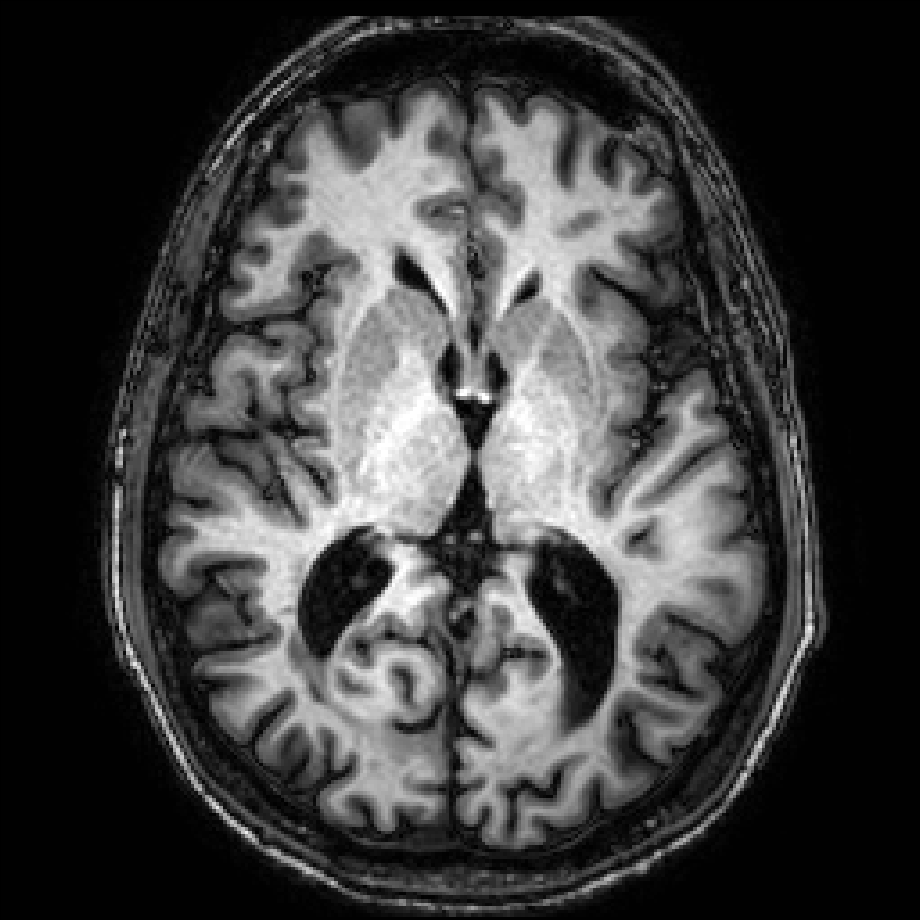
\includegraphics[width=\textwidth]{i15_training01_01_mprage.png}\caption{T1}  \label{fig:4mriT1}\end{subfigure}
  \begin{subfigure}{0.24\textwidth}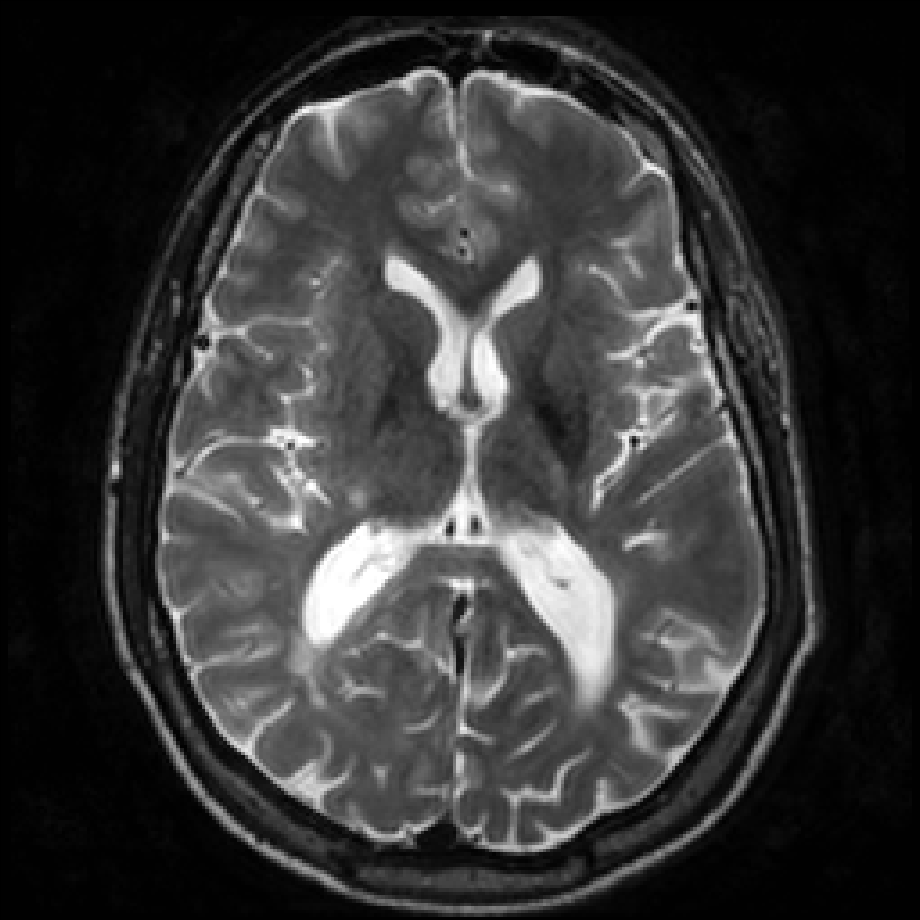
\includegraphics[width=\textwidth]{i15_training01_01_t2.png}\caption{T2}      \label{fig:4mriT2}\end{subfigure}
  \begin{subfigure}{0.24\textwidth}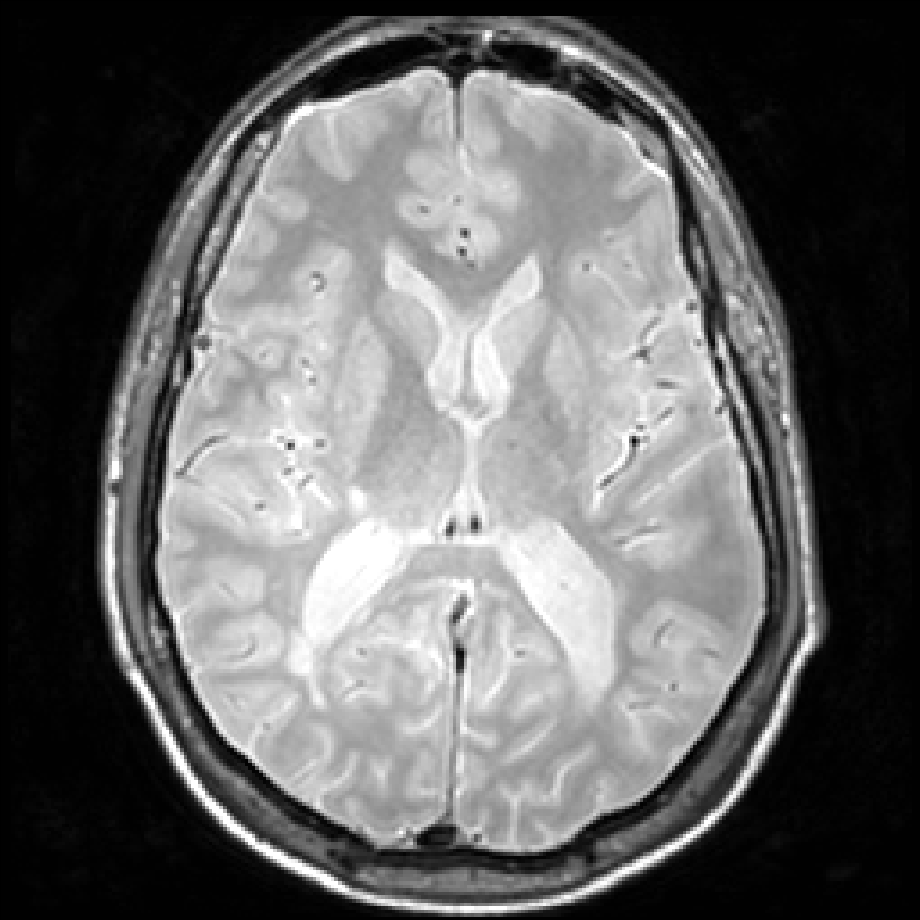
\includegraphics[width=\textwidth]{i15_training01_01_pd.png}\caption{PD}      \label{fig:4mriPD}\end{subfigure}
  \begin{subfigure}{0.24\textwidth}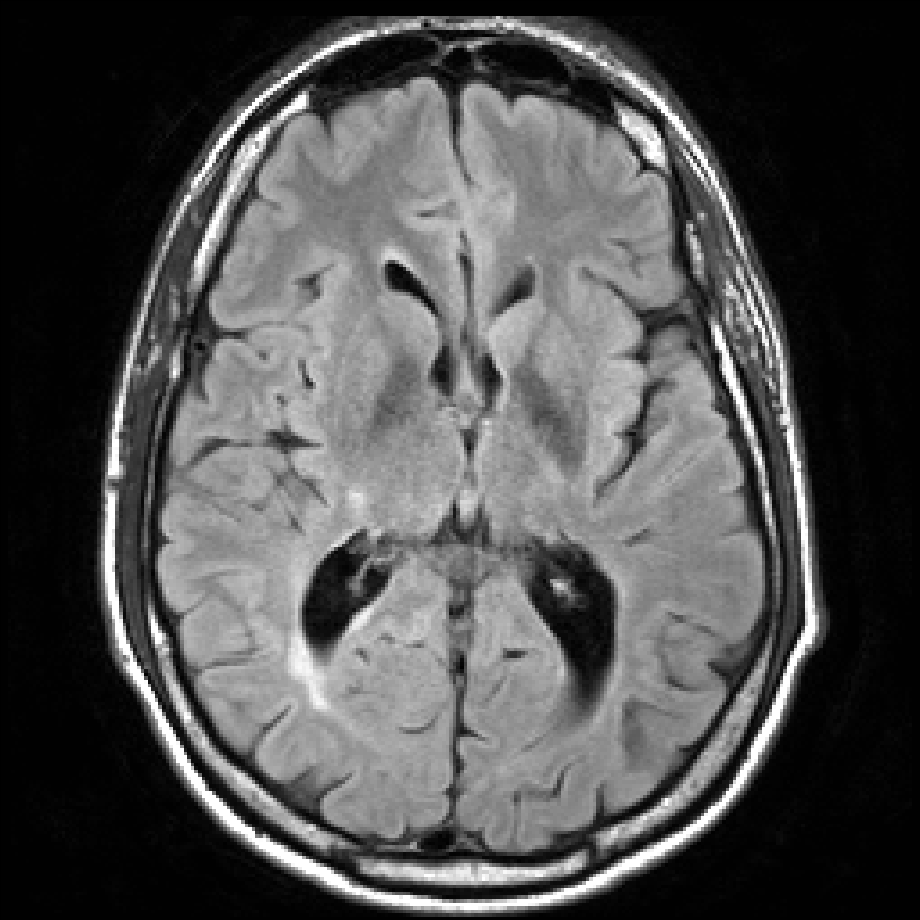
\includegraphics[width=\textwidth]{i15_training01_01_flair.png}\caption{FLAIR}\label{fig:4mriIR}\end{subfigure}
  \caption{Example MRI image set with WMH pathology; from \cite{WMHSEG2017}.}
  \label{fig:4mri}
\end{figure}
% ==================================================================================================
\subsection{White Matter Disease}\label{ss:WMD}
``Normal'' ageing of the brain is characterized by a variety of physical and cognitive changes. Memory, synaptic plasticity, and brain volume decline, with observable effects on cognitive function \cite{Peters2006,Good2002}. Brain ageing is also expedited in many patients by neurodegenerative diseases targeting the white matter, including Alzheimer's disease (AD), cerebrovascular disease, and in rare cases Multiple Sclerosis (MS). While the etiologies of these diseases are not yet fully understood, there is considerable evidence to suggest that the they are intertwined \cite{Debette2010,Conklin2014,Heppner2015,Snyder2015}.
\par
Cerebrovascular disease describes changes to blood vessels in the brain which increase the risk of ischemic injury -- a reduction in blood flow due to vessel occlusion or hemorrhage. Ischemic injuries include major events (stroke) \cite{VanderWorp2007}, transient ischemic attacks \cite{Albers2002}, and chronic hypoperfusion due to small vessel disease \cite{Pantoni2010}. In all such events, neuronal death occurs from insufficient nutrient supply \cite{VanderWorp2007}. Strokes involving major cerebral arteries can be fatal, and post-event quality of life in survivors is highly variable \cite{Prabhakaran2015}. In the less dramatic courses, clinically quiet disease progression can lead to personality changes, memory loss, and reduced cognitive ability; such changes are termed vascular dementia \cite{Roman1993}.
\par
Alzheimer's Disease is another subclass of dementia with similar symptoms; in fact it is the most common type, affecting about 6\% of the population over age 65 \cite{Burns2009}. The cause of Alzheimer's disease is hotly debated. Two 30-year-old theories linking the disease to the build up of amyloid $\beta$ protein and misfolded protein $\tau$ have been widely supported by correlational studies \cite{Masters1985,Hardy2002,Lee2011}, but have lacked clear mechanisms of injury until recently. It is now thought that amyloid $\beta$ oligomers interfere with neuronal mitochondria and synapse function, leading to cell death \cite{Kim2013,Tu2014}, while aberrant $\tau$ proteins disrupt microtubules necessary for intraneuronal transport \cite{Lee2011}. During the search for these mechanisms, competing theories implicating vascular injury \cite{Snyder2015}, immune response \cite{Heppner2015}, and blood brain barrier disruption \cite{Bell2009} have emerged, painting the picture of a more complex disease.
\par
The pathophysiology of multiple sclerosis is similarly unclear, though genetics are a necessary factor, and it is known that symptoms arise from erosion of myelin -- a fatty insulating layer surrounding axons which is critical for normal neuron firing \cite{Trapp2008}. Several theories hypothesize either that this damage is driven by autoimmune attack, followed by neuronal dysfunction and death, or that neurodegenerative changes stimulate recruitment of immune cells as part of the usual response to injury \cite{Lucchinetti2000,Trapp2008}. Recent evidence favours the former mechanism, particularly with inflammatory injury as the initiating event \cite{Ciccarelli2014,Mahad2015}.
%A helpful visualization of MS lesion progression over one year is available here\footnote{\hreftt{http://www.msdiscovery.org/sites/default/files/MGrid\_crop4\_full\_0.gif}}.
\par
Connecting all these diseases are white matter lesions (WML, \textsc{aka} Leukoariosis), which represent the macroscopic changes to brain tissue in regions of white matter damage \cite{Debette2010,Bakshi2005,Wardlaw2015}. WML are very common in elderly populations, and a small volume of lesion does not necessarily implicate one of the above diseases; in one study of 1077 subjects aged 60-90, 95\% had at least one WML \cite{DeLeeuw2001}. WML appear as bright tissue regions in T2-weighted MRI due to some combination of inflammatory injury and degradation of tissue structure \cite{Bakshi2005,Wardlaw2015}; in this imaging context, WML are often called white matter hyperintensities (WMH). Lesions are often focal, as opposed to diffuse, but there is evidence to suggest that surrounding regions of moderate hyperintensity, sometimes called ``dirty appearing white matter (DAWM)'', are also related to the diseases \cite{Ge2003}. As biomarkers of the most common WM diseases -- conditions with unsolved etiologies and inadequate treatments -- WML are of special interest to many brain researchers. The next section discusses how they are used.
% ==================================================================================================
\subsection{MRI in White Matter Disease}
MR imaging plays important roles in diagnosis and research of white matter diseases. Typical MRI protocols include T1, T2, and FLAIR sequences, though only the latter two sequences depict WML as hyperintense \cite{Simon2006,Wardlaw2013}. Depending on the disease and context, WMH can be quantified in several ways, including binary criteria (e.g. is there a lesion in a  specific location) \cite{Polman2011,Roman1993}, rating scales (e.g. a summary of several criteria) \cite{Fazekas1987}, or explicit manual segmentation of the lesions by an expert \cite{Egger2017}. 
\par
WMH are arguably most important in MS. Particularly since WMH are more specific to this disease in younger patients, WMH have long been used in the diagnosis of MS, and can even be used to replace some clinical criteria, as in the 2010 McDonald Criteria \cite{Polman2011}. MRI can also be used to discriminate between MS subtypes, which stratify disease aggression and course \cite{Polman2011,Lublin2014,Traboulsee2015}. In numerous clinical trials, WMH have also been used as biomarkers of treatment efficacy \cite{Sormani2013,Fahrbach2013,Ziemssen2015}, since WMH have been shown to be more sensitive to disease progression than clinical features in certain subtypes \cite{ORiordan1998}. In fact, despite the central role of MRI in management and research of MS, there exists a so-called ``clinico-radiological'' paradox, which is the surprisingly limited correlation between WMH and clinical MS symptoms like physical and cognitive impairment \cite{Mollison2017}. However, this only strengthens the case for continued WMH research, particularly considering the recommendations by \citeauthor{Mollison2017} in \cite{Mollison2017} to standardize image analysis in order to better understand the paradox.
\par
In dementia (including vascular and AD), WMH are used to discriminate between disease subtypes during diagnosis. For example, the presence of at least one WML was deemed \textit{necessary} for diagnosis of vascular dementia in \citeyear{Roman1993} \cite{Roman1993}, and subsequent revisions to these widely used criteria (NINCDS-ADRDA) have added this feature as an \textit{exclusionary} criteria for AD \cite{Dubois2007}. While diagnosis of additional dementia subtypes may be improved using imaging \cite{Sorbi2012,Verhagen2016}, diagnosis of the most prevalent -- AD -- continues to be based on clinical features alone \cite{McKhann2011}. As a result, WMH have not been used as an endpoint to any AD clinical trial. In fact, only recently have specific standards for use of WMH in vascular dementia studies been outlined \cite{Wardlaw2013,Wardlaw2015}, with some subsequent uptake \cite{VanWesten2016}. And yet, a \citeyear{Debette2010} meta-analysis found that WMH in brain MRI were independently correlated with stroke risk, dementia (including AD) and death \cite{Debette2010}, suggesting that much more can be done to make use of WMH as hallmarks of neurodegenerative disease.
%%%%%%%%%%%%%%%%%%%%%%%%%%%%%%%%%%%%%%%%%%%%%%%%%%%%%%%%%%%%%%%%%%%%%%%%%%%%%%%%%%%%%%%%%%%%%%%%%%%%
\section{Problem Statement}
White matter hyperintensities, as ubiquitous biomarkers of several diseases with unsolved pathophysiology, are of great interest to brain researchers. Segmentation of WMH, compared to visual rating scales, provides a finer resolution for quantification of lesion load, and gives the explicit spatial distribution of pathology. This spatial information can be very useful, since diagnostic criteria often consider lesion location \cite{Sorbi2012} and there are several correlations between lesion location and suspected etiology of WMH \cite{Kim2008,Wardlaw2015}.
\par
Unfortunately, manual segmentation of WMH is laborious, and subject to large inter- and intra-rater variability, as reported in several works. Table \ref{tab:interrater-cite} summarizes these reports, where similarity index (SI $\in [0,1]$) is a measure of voxel-wise agreement, and interclass correlation coefficient (ICC $\in [0,1]$) measures total volume agreement (cf. \S\ \ref{ss:metrics} for definitions). Table \ref{tab:interrater-cite} also gives the results using four semi-automated approaches, since these methods are reported to reduce variability and task time over strictly manual segmentation. Yet, for very large scale research studies, any approach requiring human intervention would be prohibitively time consuming and subjective. 
\par 
Therefore, a fully automated algorithm to segment WMH in MRI is required. Such an algorithm would have, by construction, perfect repeatability, and consistent bias -- which is especially important for perceiving small changes in longitudinal studies \cite{MSISBI2015}. Additionally, while an automated approach may not necessarily be faster than manual or semi-automatic segmentation on a per-case basis, it could be run on several computers in parallel, yielding significant overall speed up.
\par
Furthermore, while T1, T2, and FLAIR sequences are typically recommended for both MS and dementia investigations \cite{Simon2006,Wardlaw2013,Traboulsee2015}, FLAIR sequences are at least as sensitive as T2 images for the detection of WML\footnote{Early studies exploring the utility of FLAIR sequences may contradict this claim \cite{Okuda1999,Rovaris2000}, but FLAIR imaging has since improved \cite{Wardlaw2015}.}. As noted above, FLAIR images also have the advantage of easily distinguishing WMH from confounding CSF hyperintensity, which is important for highly prevalent periventricular lesions, and also for excluding lacunar infarcts \cite{Bakshi2001,Barkhof2002}. Consequently, it should be feasible to detect WMH using FLAIR MRI alone. This has several advantages, including minimizing the required MR sequences available during retrospective analyses, decreasing cost and scan time in prospective studies, and eliminating the need for intra-subject image registration if sequences are acquired at different resolutions (as is often the case).
\par
\begin{table}[h]
  \caption{Mean inter-rater agreement measures for manual and semi-automated WMH segmentation reported in previous works.}
  \centering
  \begin{tabular}{lccccc}
    \hline
                                    &         Ref          & Raters &    Data    &  SI  & ICC  \\ \hline
    \multirow{4}{*}{Manual}         & \cite{Harmouche2006} &   5    & 10 images  & 0.64 & ---  \\
                                    &  \cite{DeBoer2009b}  &   2    &  6 images  & 0.75 & ---  \\
                                    & \cite{Steenwijk2013} &   2    & 120 slices & 0.83 & 0.96 \\
                                    &   \cite{Egger2017}   &   3    & 50 images  & 0.66 & 0.97 \\ \hline
    \multirow{4}{*}{Semi-Automated} &   \cite{Payne2002}   &   1    & 16 images  & ---  & 0.99 \\
                                    &  \cite{Ghazel2006}   &   1    &  2 images  & 0.70 & ---  \\
                                    &  \cite{Kawata2010}   &   1    & 33 slices  & 0.78 & ---  \\
                                    &   \cite{Iorio2013}   &   2    & 30 images  & 0.78 & ---  \\ \hline
  \end{tabular}
  \label{tab:interrater-cite}
\end{table}
% ==================================================================================================
\subsection{Objective}
The primary objective of this thesis is to develop an algorithm for fully automatic segmentation of WMH, using FLAIR MRI alone. Secondary objectives include:
\begin{itemize}
  \item analysis of the limitations of prior work in this area;
  \item exploration and definition of appropriate cross validation techniques for the task;
  \item validation of the proposed algorithm on a large and heterogeneous database of FLAIR images.
\end{itemize}
% ==================================================================================================
\subsection{Challenges to Automatic Segmentation}\label{ss:autochallenges}
While fully automated segmentation of WMH is attractive, translation of expert knowledge into algorithmic constructs is difficult, and often requires assumptions which induce sensitivity of the model to seemingly extraneous image features. Moreover, human understanding of MR acquisition physics help radiologists to distinguish WML from image artifacts. Thus, there are several challenges to automatic segmentation. These can be summarized as follows:
\begin{enumerate}[itemsep=0pt,topsep=0pt]
  \item \label{chauto:overlap}     \textbf{Overlapping distributions:} \\
  Using the relaxation constants in Table \ref{tab:t1t2tissues} in conjunction with the FLAIR signal equation (\ref{eq:MRI-IR}), the predicted intensity distributions of GM and WMH can overlap, depending on the choice of TE, TR, and TI (cf. Table \ref{tab:database} for typical values and \S\ \ref{s:simflair} for modelling). As a result, the intensity of image voxels alone cannot be used to determine their class \cite{Mortazavi2012}.
  \item \label{chauto:bias}        \textbf{Bias field:} \\
  The most common image artifact in MRI is due to inhomogeneity in the main magnetic field during acquisition, which is difficult to eliminate in strong electromagnets; this creates a low frequency variation in signal intensity over the imaged volume \cite{Juntu2005}. The overall effect is that the same tissues may have different graylevels in different locations, further confounding the uniqueness of WMH graylevels \cite{Wardlaw2015}.
  \item \label{chauto:dawm}        \textbf{DAWM:} \\
  Most of the inter-rater disagreement in manual segmentation of WMH is arguably due to ambiguity of pathological extent at the lesion borders, where the core lesion meets so-called DAWM \cite{Ge2003}. If human judgement of this boundary is difficult, then programmatic definitions could be expected to be similarly challenged.
  \item \label{chauto:pva}         \textbf{Partial volume effect:} \\
  With finite image resolution, voxels located on tissue boundaries will inevitably contain tissues of two or more tissues. This is known as partial volume effect (PVE), and the resulting signal intensity can be modelled as a linear mixture of the components \cite{Santago1995}. \citeauthor{Niessen1999} \cite{Niessen1999} show that inadequate modelling of PVE can result in significant errors in tissue segmentation, though the widely reported 30\% figure from this work is derived from unrealistic conditions.
  \item \label{chauto:artifacts}   \textbf{Artifacts:} \\
  Due to the complexity of signal acquisition, there are several artifacts which can manifest in MR images. Artifacts which appear hyperintense in T2 images (including FLAIR) are of particular importance to the current work, since these confound bright pathologies, and must therefore be excluded using other features; the most notable artifacts include \cite{Wardlaw2015}:
  \begin{itemize}[itemsep=0pt,topsep=0pt]
    \item CSF flow artifacts -- ventricular hyperintensities resulting from movement of magnetically polarized CSF fluid during the inversion interval (cf. \S\ \ref{ss:mri}) \cite{Bakshi2000};
    \item Perivascular spaces -- minuscule spaces adjacent to cerebral vessels whose properties differ from ventricular and sulcal CSF, and are therefore not attenuated in FLAIR images \cite{Wardlaw2015};
    \item Motion artifacts -- artifacts which originate during frequency-domain encoding of spatial image content with subject motion, which is more common in MRI due to long acquisition times (several minutes); these typically manifest as high frequency ``ringing'' artifacts \cite{Zaitsev2015}.
 %  \item Recent small subcortical infarcts;
  \end{itemize}
  \item \label{chauto:variability} \textbf{Image variability:} \\
  There are a large number variable characteristics of MR images; some of these can be selected at acquisition time based on time constraints, and physician preferences, while others are immutable. ``Image variability'' is taken to comprise:
  \begin{itemize}[itemsep=0pt,topsep=0pt]
    \item differences in image contrasts (and tissue graylevel distributions), due to selection of MRI parameters;
    \item differences in image resolution (voxel size);
    \item differences in MRI scanner, including field strength and proprietary image reconstruction;
    \item inter-subject anatomical variability and lesion heterogeneity.
  \end{itemize}
  Modelling this immense gamut of possible image characteristics (e.g. using parametric distributions or task-specific assumptions) represents perhaps the most challenging aspect to automated image analysis. Some specific impacts will be further discussed in \S\ \ref{ss:priorlimits}.
\end{enumerate}
An optimal WMH segmentation algorithm will therefore consider and address each of these challenges.
%%%%%%%%%%%%%%%%%%%%%%%%%%%%%%%%%%%%%%%%%%%%%%%%%%%%%%%%%%%%%%%%%%%%%%%%%%%%%%%%%%%%%%%%%%%%%%%%%%%%
\section{Prior Work}
This endeavour is far from original. Efforts to automate segmentation of WMH date back to \citeyear{Kapouleas1990} \cite{Kapouleas1990} and the task has been the subject of several major reviews in \citeyear{Llado2012} \cite{Llado2012,Mortazavi2012}, \citeyear{Garcia-Lorenzo2013} \cite{Garcia-Lorenzo2013}, and \citeyear{Caligiuri2015} \cite{Caligiuri2015}. The task has also been featured in four international competitions at the MICCAI (Medical Image Computing and Computer Assisted Intervention) Conference -- 2008 \cite{MSSEG2008}, 2016 \cite{MSSEG2016}, and 2017 \cite{WMHSEG2017} -- and the ISBI (International Symposium on Biomedical Imaging) Conference -- 2015 \cite{MSISBI2015} -- in which researchers vie to produce the best segmentation algorithms (for more on competitions, cf. \S\ \ref{ss:competitions}). A summary of many of the proposed approaches is given in Table \ref{tab:wmlsegtable}\footnote{A more detailed and interactive version of this table is available at \hreftt{www.uoguelph.ca/~jknigh04/wmlseg/table.html}}. Below, the most important contributions in this area are introduced and summarized.
\begin{table}
  \caption{Summary of previous approaches to WMH segmentation with respect to image variability and reported performance (SI).}
  \footnotesize{\centering{{\setmaxcitenames{1}
\begin{tabular}{lcclcccc}
	\toprule
  \# & Ref. & Year & Authors          &     MRI Sequences     & I   & S  & SI  \\
  \midrule
	\citefortable{VanLeemput2001}       &      T1, T2, PD       & 20  & 1  & 0.51 \\
	\citefortable{Jack2001}             &         FLAIR         & 39  & 1  &      \\
	\citefortable{Zijdenbos2002}        &        T1, T2         & 10  & 1  & 0.6  \\
	\citefortable{Anbeek2004}           & T1, T2, PD, FLAIR, IR & 20  & 1  & 0.61 \\
	\citefortable{Anbeek2005}           & T1, T2, PD, FLAIR, IR & 10  & 1  & 0.78 \\
	\citefortable{Admiraal-Behloul2005} &     T2, PD, FLAIR     & 100 & 1  & 0.75 \\
	\citefortable{Lao2006}              &   T1, T2, PD, FLAIR   & 45  & 1  &      \\
	\citefortable{Wu2006}               &      T1, T2, PD       & 12  & 1  &      \\
	\citefortable{Sajja2006}            &     T2, PD, FLAIR     & 23  & 1  & 0.78 \\
	\citefortable{Harmouche2006}        &      T1, T2, PD       & 10  & 1  & 0.61 \\
	\citefortable{Khayati2008}          &         FLAIR         & 20  & 1  & 0.75 \\
	\citefortable{Wels2008}             &     T1, T2, FLAIR     &  6  & 1  & 0.57 \\
	\citefortable{Herskovits2008}       &   T1, T2, PD, FLAIR   & 42  & 2  & 0.6  \\
	\citefortable{Bricq2008}            &       T2, FLAIR       & 25  & 2  &      \\
	\citefortable{Dyrby2008}            &     T1, T2, FLAIR     & 362 & 10 & 0.56 \\
	\citefortable{Souplet2008}          &     T1, T2, FLAIR     & 25  & 2  &      \\
	\citefortable{DeBoer2009b}          &     T1, PD, FLAIR     & 20  & 2  & 0.72 \\
	\citefortable{Garcia-Lorenzo2009}   &      T1, T2, PD       & 10  & 1  & 0.63 \\
	\citefortable{Akselrod-Ballin2009}  &   T1, T2, PD, FLAIR   & 41  & 1  & 0.53 \\
	\citefortable{Schwarz2009}          &      T1, T2, PD       & 165 & 2  &      \\
	\citefortable{Gibson2010}           &     T1, T2, FLAIR     & 18  & 1  & 0.81 \\
	\citefortable{Shiee2010}            &       T1, FLAIR       & 10  & 1  & 0.63 \\
	\citefortable{Scully2010}           &     T1, T2, FLAIR     & 17  & 1  &      \\
	\citefortable{Garcia-Lorenzo2011}   &     T1, T2, FLAIR     & 10  & 1  & 0.65 \\
	\citefortable{Geremia2011}          &     T1, T2, FLAIR     & 20  & 2  &      \\
	\citefortable{Smart2011}            &       T1, FLAIR       & 30  & 1  &      \\
	\citefortable{Samaille2012}         &       T1, FLAIR       & 67  & 6  & 0.72 \\
	\citefortable{Khademi2012}          &         FLAIR         & 24  & 1  & 0.83 \\
	\citefortable{Schmidt2012}          &       T1, FLAIR       & 53  & 1  & 0.75 \\
	\citefortable{Abdullah2012}         &     T1, T2, FLAIR     & 61  & 3  &      \\
	\citefortable{Sweeney2013}          &   T1, T2, PD, FLAIR   & 111 & 1  & 0.61 \\
	\citefortable{Datta2013}            &     T1, T2, FLAIR     & 90  & 3  &      \\
	\citefortable{Steenwijk2013}        &       T1, FLAIR       & 40  & 2  & 0.8  \\
	\citefortable{Khademi2014}          &         FLAIR         & 25  & 1  & 0.78 \\
	\citefortable{Ithapu2014}           &       T1, FLAIR       & 38  & 1  & 0.67 \\
	\citefortable{Yoo2014}              &         FLAIR         & 32  & 2  & 0.76 \\
	\citefortable{Harmouche2015}        &   T1, T2, PD, FLAIR   & 100 & 35 & 0.56 \\
	\citefortable{Guizard2015}          &   T1, T2, PD, FLAIR   & 108 & 32 & 0.6  \\
	\citefortable{Jain2015}             &       T1, FLAIR       & 20  & 1  & 0.67 \\
	\citefortable{Tomas-Fernandez2015}  &     T1, T2, FLAIR     & 51  & 2  &      \\
	\citefortable{Wang2015}             &     T1, T2, FLAIR     & 70  & 2  & 0.84 \\
	\citefortable{Roy2015}              &         FLAIR         & 38  & 3  & 0.56 \\
	\citefortable{Brosch2015}           &     T1, T2, FLAIR     & 20  & 2  & 0.36 \\
	\citefortable{Fartaria2015}         &         FLAIR         & 39  & 1  & 0.55 \\
	\citefortable{Deshpande2015}        &   T1, T2, PD, FLAIR   & 52  & 1  & 0.5  \\
	\citefortable{Roura2015}            &       T1, FLAIR       & 20  & 2  & 0.34 \\
	\citefortable{Knight2016a}          &         FLAIR         & 15  & 3  & 0.7  \\
	\citefortable{Mechrez2016}          &     T1, T2, FLAIR     & 20  & 2  & 0.31 \\
	\citefortable{Strumia2016}          &       T1, FLAIR       & 20  & 3  & 0.52 \\
	\citefortable{Griffanti2016}        &       T1, FLAIR       & 130 & 2  & 0.76 \\
	\citefortable{Valverde2016}         &       T1, FLAIR       & 33  & 2  &      \\
	\citefortable{Dadar2017}            &       T1, FLAIR       & 80  & 3  & 0.62 \\
	\citefortable{Zhan2017}             &     T1, T2, FLAIR     & 50  & 2  & 0.76 \\ \bottomrule
\end{tabular}
}\\[0.5em]
\raggedright{\footnotesize{Abbreviations.
I\@: number of MR image sets used for validation;
S\@: number of MRI scanners used for validation;
SI\@: reported validation similarity index.}}
}}
  \label{tab:wmlsegtable}
\end{table}
% ==================================================================================================
\subsection{Segmentation Models \& Features}
Segmentation models represent a mapping from the content of an observed image to an image of labels or classes -- in this case, tissues. The output class image comprises an estimated label for each observed voxel, or, in probabilistic models, the probability of each class for each voxel. As in many classification problems, models can be described as either supervised or unsupervised. Supervised models have relatively large capacity to model arbitrary mappings, but learn a mapping relevant to the current task using feedback from labelled examples (i.e. by a human). Unsupervised models, by contrast, are usually problem-specific, and leverage prior knowledge and the image features to predict the label image; they do not require labelled data for optimization, at least in principle. 
\par
Features used for segmentation can be derived from individual voxels (e.g. graylevel), groups of voxels (e.g. local mean graylevel), the entire image (e.g. a histogram feature), spatial location (e.g. coordinates in a standardized space), or prior knowledge (e.g. class prior probability). It is often useful to imagine the space spanned by all possible values of all features; this is called the feature space. Each observed voxel, having a unique value for each feature, therefore represents a unique location in this space. The task of segmentation is therefore to divide the feature space into subspaces corresponding to each class. In probabilistic models, these subspaces are better described as distributions of each class over the features.
\par
Previous approaches to WMH segmentation have generally employed three types of features:
\begin{itemize}
  \item \textbf{Graylevel:} graylevels of MRI sequences, often following standardization (e.g. T1, T2, PD, FLAIR);
  \item \textbf{Prior:} prior tissue probability, often derived from a coregistered prior image (e.g. ICBM \cite{Mazziotta2001});
  \item \textbf{Spatial:} spatial location, often normalized to a common space (e.g. $\x_1, \x_2, \x_3$).
\end{itemize}
Additional features types are rarely used, since the combination of the above features are typically the only features employed by human raters. At least one graylevel feature is always used, since it is the only image-specific information (i.e. the evidence).
% ==================================================================================================
\subsection{Proposed Methods}\label{ss:priorproposed}
The specific methods proposed for WMH segmentation are now reviewed.\footnote{This section copied verbatim from a paper in submission \cite{Knight2017a} -- is this allowed?}
% --------------------------------------------------------------------------------------------------
\newcommand{\priorworksub}[1]{\subsubsection{#1}}
% --------------------------------------------------------------------------------------------------
\priorworksub{Thresholding Techniques}
Since WMH are brighter than healthy brain tissue in FLAIR images, many unsupervised works have used thresholding of FLAIR intensities as the initial lesion segmentation.
For example, in the works by~\citeauthor{Jack2001}~\cite{Jack2001},~\citeauthor{DeBoer2009b}~\cite{DeBoer2009b}, and~\citeauthor{Smart2011},~\cite{Smart2011} optimal FLAIR thresholds are empirically estimated relative to histogram statistics, though~\citeauthor{DeBoer2009b} use only estimated GM voxels in the histogram.
\citeauthor{Gibson2010} use a conservative FLAIR threshold initially, but then classify the remaining voxels using Fuzzy C Means clustering~\cite{Gibson2010}.
\citeauthor{Samaille2012} use nonlinear diffusion filtering and watershed segmentation, before classifying candidate regions based on a FLAIR image threshold.
\citeauthor{Yoo2014} estimate the optimal threshold for FLAIR images using histogram statistics, derived from a regression model primarily considering the total lesion load~\cite{Yoo2014}.
In works by~\citeauthor{Khademi2014}, a peak in the conditional probability of edge content on graylevel is used to predict the transition between healthy tissue and lesion~\cite{Khademi2014,Khademi2015,Knight2016a}.
% --------------------------------------------------------------------------------------------------
\priorworksub{Mixture Models}
Most other unsupervised approaches are probabilistic models, often framed as a mixture model.
The work by~\citeauthor{VanLeemput2001}~\cite{VanLeemput2001} uses a similar framework as the early work by~\citeauthor{Ashburner1997}~\cite{Ashburner1997}, later incorporated into the SPM ``segment'' tool~\cite{Ashburner2005}, which jointly estimates Gaussian graylevel distributions for each tissue class, and also bias field, using expectation maximization. In the model by~\citeauthor{VanLeemput2001}, distribution parameters are estimated using outlier-insensitive estimators, and WMH are derived from model outliers using heuristic rules. The predicted classes are also smoothed spatially using a Markov Random Field (MRF).
\par
Similar works by~\citeauthor{Bricq2008}~\cite{Bricq2008},~\citeauthor{Schmidt2012}~\cite{Schmidt2012},~\citeauthor{Jain2015}~\cite{Jain2015}, and~\citeauthor{Roura2015}~\cite{Roura2015} use parametric mixture models to predict WMH as model outliers, and all but~\cite{Roura2015} embed the model in a MRF\@.
~\citeauthor{Khayati2008}~\cite{Khayati2008} and~\citeauthor{Subbanna2009}~\cite{Subbanna2009} also use MRF-constrained mixture models, but model WMHs as a Gaussian-distributed tissue class, rather than as outliers.
In the works by~\citeauthor{Harmouche2006}, parametric distributions are also used to model lesions, but such distributions are parameterized independently per brain region, in order to reflect lobe heterogeneity; a MRF is again used for regularization~\cite{Harmouche2006,Harmouche2015}.
\citeauthor{Schwarz2009} again employ a Bayesian MRF model, but use lognormal distributions for WM and WMH~\cite{Schwarz2009}.
\citeauthor{Souplet2008} use an augmented mixture model which includes partial volume averaging classes and an outlier class to perform initial brain tissue segmentation; WMH are subsequently classified using a FLAIR intensity threshold after contrast enhancement~\cite{Souplet2008}. 
The work by~\citeauthor{Herskovits2008} is much the same, but uses statistical information from training data to classify lesions (i.e.\ it is supervised)~\cite{Herskovits2008}.
More recently, Graph-Cuts have been used in conjunction with mixture models, as in the works by~\citeauthor{Garcia-Lorenzo2009}~\cite{Garcia-Lorenzo2009},~\citeauthor{Tomas-Fernandez2015}~\cite{Tomas-Fernandez2015}, and~\citeauthor{Strumia2016}~\cite{Strumia2016}.
\par
The Lesion-TOADS method by~\citeauthor{Shiee2010}~\cite{Shiee2010}, a lesion-specific adaptation of the TOADS algorithm~\cite{Bazin2008}, presents an entirely new non-Gaussian paradigm for modelling class distributions, and incorporates topological energies in the objective function.
Other proposed unsupervised methods have used clustering by Fuzzy C-Means, including the works by~\citeauthor{Admiraal-Behloul2005}~\cite{Admiraal-Behloul2005},~\citeauthor{Gibson2010}~\cite{Gibson2010}, and~\citeauthor{Valverde2016}~\cite{Valverde2016}.
% --------------------------------------------------------------------------------------------------
\priorworksub{Classic Supervised Methods}
Many early supervised methods used K-Nearest Neighbours (K-NN) for voxel-wise WMH classification.
\citeauthor{Anbeek2005} used a K-NN model with features derived from spatial coordinates and voxel intensities from several modalities~\cite{Anbeek2004,Anbeek2005}.
In the works by~\citeauthor{Wu2006}~\cite{Wu2006},~\citeauthor{Steenwijk2013}~\cite{Steenwijk2013}, and~\citeauthor{Fartaria2015}~\cite{Fartaria2015}, spatial coordinates are substituted for tissue priors as K-NN features.
In the recently proposed BIANCA algorithm by~\citeauthor{Griffanti2016}~\cite{Griffanti2016}, spatial coordinates are added back, along with some patch-based features.
\par
Other works have also explored Support Vector Machines (SVM) for classification.
The works by~\citeauthor{Lao2006}~\cite{Lao2006},~\citeauthor{Abdullah2012}~\cite{Abdullah2012}, and~\citeauthor{Scully2010}~\cite{Scully2010} each use a selection of intensity features, neighbouring intensities, tissue priors, morphological, and texture features with an SVM classifier.
Several more recent works have used decision tree-based classifiers, including Random Forest (RF) and AdaBoost.
\citeauthor{Akselrod-Ballin2009}~\cite{Akselrod-Ballin2009} employ over 30 features for multi-scale image representation and classify voxels using RF\@.
Both~\citeauthor{Geremia2011}~\cite{Geremia2011} and~\citeauthor{Roy2015}~\cite{Roy2015} use a combination of intensity and tissue prior features to train a RF classifier, whereas~\citeauthor{Wels2008}~\cite{Wels2008} use a large number of Haar-like features to train an AdaBoost model.
\citeauthor{Ithapu2014}~\cite{Ithapu2014} explore the use of texton features in both SVM and RF models.
\par
Logistic regression models have also gained popularity recently.
In the OASIS model by~\citeauthor{Sweeney2013}~\cite{Sweeney2013}, image intensities from T1, T2, PD, and FLAIR sequences are used individually, in multiplicative combination, and with Gaussian blurring as predictors for a global set of logistic regression parameters.
In the work by~\citeauthor{Zhan2017}~\cite{Zhan2017}, a similar logistic model is fitted using only the raw T1, T2, and FLAIR intensities, while bias correction is performed as preprocessing and spatial smoothness using MRF post processing.
In the work by~\citeauthor{Dadar2017}~\cite{Dadar2017}, spatial and intensity features from a flexible selection of MR sequences are used to train a linear regression model, the results of which are thresholded to give the lesion prediction.
Still more works have proposed other supervised models, including nonparametric Parzen classifiers~\cite{Sajja2006}.
% --------------------------------------------------------------------------------------------------
\priorworksub{Deep Learning}
A number of deep learning approaches have also been proposed, though their permeation in this problem space is surprisingly limited.
Both~\citeauthor{Zijdenbos2002}~\cite{Zijdenbos2002} and~\citeauthor{Dyrby2008}~\cite{Dyrby2008} train fully-connected voxel-wise Neural Networks with a selection of intensity, spatial, and tissue prior features to predict the lesion class.
In contrast,~\citeauthor{Brosch2015}~\cite{Brosch2015} construct a more modern deep convolutional model, which is capable of capturing both local and global dependencies.
% --------------------------------------------------------------------------------------------------
\priorworksub{External Toolboxes}
Many of the proposed methods use registration, brain extraction, bias field correction, and segmentation tools available in freely available toolkits; these include the SPM\footnote{\hreftt{http://www.fil.ion.ucl.ac.uk/spm/}} toolkit
~\cite{Sajja2006,Dyrby2008,Akselrod-Ballin2009,Smart2011,Schmidt2012,Yoo2014,Ithapu2014,Roy2015,Valverde2016} and the
FSL\footnote{\hreftt{https://fsl.fmrib.ox.ac.uk/fsl/}} toolkit
~\cite{Herskovits2008,Gibson2010,Datta2013,Steenwijk2013,Sweeney2013,Roy2015,Wang2015,Griffanti2016,Zhan2017},
as well as bias correction by the
N3/4
\footnote{\hreftt{https://www.slicer.org/wiki/Documentation/4.6/Modules/N4ITKBiasFieldCorrection}} 
~\cite{Tustison2010}
algorithm
~\cite{Zijdenbos2002,Harmouche2006,Fartaria2015,Guizard2015,Harmouche2015,Mechrez2016,Valverde2016,Dadar2017,Zhan2017}.
% --------------------------------------------------------------------------------------------------
% ==================================================================================================
\subsection{Limitations}\label{ss:priorlimits}
Despite over 50 proposed algorithms and several competitions, no WMH segmentation algorithm has clearly emerged the superior method, nor has any been taken up for use in the wider research community. This is contrasted with other neuroimaging tasks, where several robust tools noted above are now regularly used in analysis pipelines -- e.g. N3/4 \cite{Tustison2010} for bias field correction, BET for brain extraction \cite{Smith2002a}, SPM Segment \cite{Ashburner2005} / FSL FAST \cite{Zhang2001} for healthy brain segmentation, SPM Coregister \cite{Ashburner2005} / FSL FLIRT \cite{Jenkinson2001} for registration. We hypothesize two reasons for this gap in WMH segmentation tools.
\par
First, very few of the proposed methods have been released as either open-source code or compiled applications. Researchers may not want to release source code for reasons related to intellectual property, or the additional work of ensuring robustness and writing documentation. Yet the field of deep learning illustrates how these practices can accelerate progress in the field enormously. Similarly, compiling applications for cross-platform compatibility is no small feat, though there are many examples for SPM extensions\footnote{\hreftt{http://www.fil.ion.ucl.ac.uk/spm/ext/}}, as well as events by NA-MIC (National Alliance for Medical Image Computing) for development of 3D Slicer modules\footnote{\hreftt{https://na-mic.org/wiki/Events}}.
\par
Second, very few of the WMH segmentation methods have been validated on large, multi-centre databases: of the 53 works reviewed (Table \ref{tab:wmlsegtable}), less than half use more than one scanner for validation, and only 4 use more than three. As noted in \S\ \ref{ss:autochallenges}, there are several sources of image variability in MRI, and both supervised and unsupervised methods can be sensitive to these factors, as noted by several authors \cite{Llado2012,Sweeney2013,Dadar2017}. Therefore, while many of the proposed methods may be of use for in-house work (i.e. with images from a consistent source), there can be little confidence that they will perform as reported on data from new sources (generalization performance).
\par
In supervised models, graylevel features must be standardized, since the MRI intensity scale is not consistent across scanners or scan parameters, due to the complexity of signal acquisition \cite{Nyul1999}. However, this is not an easy task. For example, \citeauthor{Steenwijk2013} validate a supervised WMH segmentation algorithm using same-scanner training and testing for two different scanners independently (mean SI = 0.75, 0.84), after variance scaling of intensity features \cite{Steenwijk2013}. Yet, a follow-up experiment which saw the method trained on one scanner and tested on the other showed a precipitous drop in performance to mean SI = 0.50. 
\par
Unsupervised models also have parameters which can be inadvertently over-tuned to data from one or two sources. For example, mixture models which classify lesions as outliers often employ an outlier definition which depends on mixture model parameters (e.g. tissue graylevel mean and variance), which in turn are subject to MR slice thickness, noise level, and contrast \cite{VanLeemput2001,Souplet2008,Garcia-Lorenzo2011,Roura2015}. Graylevel thresholding techniques \cite{Jack2001,Smart2011,Samaille2012,Schmidt2012,Khademi2014} are similarly affected by changes in image properties.
\par
It is worth noting three works\footnotemark\ which run counter to this trend, demonstrating robust validation of their proposed methods. These works are summarized in Table \ref{tab:priorworkval}. Perhaps not surprisingly, these papers report lower performance (mean SI $\le 0.60$) than other works; as a result, these algorithms would not likely be used for clinical research. Yet, even these works do not optimally estimate the model generalization performance for data from new scanners, as will be discussed in \S\ \ref{s:CVframeworks}. Moreover, the proposed algorithms in these papers require at least three MRI sequences, which fails the objectives of the current work.
\footnotetext{The work by \citeauthor{Samaille2012} (\citeyear{Samaille2012}) \cite{Samaille2012} is also a good candidate, having used 6 scanners for validation; however, 43 of the 67 images (64\%) come only from one scanner, reducing the robustness of generalization results.}
\begin{table}[h]
  \newcommand{\citefortablev}[1]{{\cite{#1}}&{\citeyear{#1}}&{\citeauthor{#1}}}
  \caption{Works demonstrating excellent validation of a WMH segmentation algorithm.}\label{tab:priorworkval}
  \centering
    \begin{tabular}{cclccc}
      \hline
      Ref.&Year&Authors&I&S&SI
      \\\hline
      \citefortablev{Dyrby2008} & 362 & 10 & 0.56 \\
      \citefortablev{Guizard2015} & 108 & 32 & 0.60 \\
      \citefortablev{Harmouche2015} & 100 & 35 & 0.56 \\
      \hline
    \end{tabular}
  \tablepost{
    Abbreviations. 
    I: number of MR image sets used for validation;
    S: number of MRI scanner-parameter combinations used for validation;
    SI: reported validation similarity index.}
\end{table}
%%%%%%%%%%%%%%%%%%%%%%%%%%%%%%%%%%%%%%%%%%%%%%%%%%%%%%%%%%%%%%%%%%%%%%%%%%%%%%%%%%%%%%%%%%%%%%%%%%%%
\section{Contributions}
This thesis therefore aims to produce a WMH segmentation algorithm which can be used on FLAIR MRI from any source, and to characterize the expected performance on unseen data. The major contributions are as follows:
\begin{enumerate}
  \item A review and critique of the previously proposed WMH segmentation algorithms, especially with respect to expected performance on unseen data;
  \item Voxel-Wise Logistic Regression (VLR): a new FLAIR-only WMH segmentation algorithm;
  \item Leave-One-Source-Out Cross Validation (LOSO-CV): a validation framework which accurately characterizes the generalization performance of medical image analysis methods;
  \item Extensive validation of the proposed method and its components.
\end{enumerate}
The remainder of this thesis is organized as follows:
Chapter 2 motivates and develops the voxel-wise logistic regression model, including expected challenges and solutions with this approach;
Chapter 3 explores optimization of model components through experiment, and then presents segmentation performance results under various cross validation schemes;
Chapter 4 discusses the performance results, summarizes the contributions, and highlights avenues of future work.
% --------------------------------------------------------------------------------------------------
% ==================================================================================================
%%%%%%%%%%%%%%%%%%%%%%%%%%%%%%%%%%%%%%%%%%%%%%%%%%%%%%%%%%%%%%%%%%%%%%%%%%%%%%%%%%%%%%%%%%%%%%%%%%%%
